\documentclass{beamer}

\pdfmapfile{+sansmathaccent.map}


\mode<presentation>
{
	\usetheme{Warsaw} % or try Darmstadt, Madrid, Warsaw, Rochester, CambridgeUS, ...
	\usecolortheme{seahorse} % or try seahorse, beaver, crane, wolverine, ...
	\usefonttheme{serif}  % or try serif, structurebold, ...
	\setbeamertemplate{navigation symbols}{}
	\setbeamertemplate{caption}[numbered]
} 


%%%%%%%%%%%%%%%%%%%%%%%%%%%%
% itemize settings


%%%%%%%%%%%%%%%%%%%%%%%%%%%%
% itemize settings

\definecolor{myhotpink}{RGB}{255, 80, 200}
\definecolor{mywarmpink}{RGB}{255, 60, 160}
\definecolor{mylightpink}{RGB}{255, 80, 200}
\definecolor{mypink}{RGB}{255, 30, 80}
\definecolor{mydarkpink}{RGB}{155, 25, 60}

\definecolor{mypaleblue}{RGB}{240, 240, 255}
\definecolor{mylightblue}{RGB}{120, 150, 255}
\definecolor{myblue}{RGB}{90, 90, 255}
\definecolor{mygblue}{RGB}{70, 110, 240}
\definecolor{mydarkblue}{RGB}{0, 0, 180}
\definecolor{myblackblue}{RGB}{40, 40, 120}

\definecolor{myblackturquoise}{RGB}{5, 53, 60}
\definecolor{mydarkdarkturquoise}{RGB}{8, 93, 110}
\definecolor{mydarkturquoise}{RGB}{28, 143, 150}
\definecolor{mypaleturquoise}{RGB}{230, 255, 255}
\definecolor{myturquoise}{RGB}{48, 213, 200}

\definecolor{mygreen}{RGB}{0, 200, 0}
\definecolor{mydarkgreen}{RGB}{0, 120, 0}
\definecolor{mygreen2}{RGB}{245, 255, 230}

\definecolor{mygrey}{RGB}{120, 120, 120}
\definecolor{mypalegrey}{RGB}{160, 160, 160}
\definecolor{mydarkgrey}{RGB}{80, 80, 160}

\definecolor{mydarkred}{RGB}{160, 30, 30}
\definecolor{mylightred}{RGB}{255, 150, 150}
\definecolor{myred}{RGB}{200, 110, 110}
\definecolor{myblackred}{RGB}{120, 40, 40}


\definecolor{myblackmaroon}{RGB}{50, 0, 15}

\definecolor{mygreen}{RGB}{0, 200, 0}
\definecolor{mygreen2}{RGB}{205, 255, 200}

\definecolor{mydarkcolor}{RGB}{60, 25, 155}
\definecolor{mylightcolor}{RGB}{130, 180, 250}

\setbeamertemplate{itemize items}[default]

\setbeamertemplate{itemize item}{\color{myblackmaroon}$\blacksquare$}
\setbeamertemplate{itemize subitem}{\color{mydarkdarkturquoise}$\blacktriangleright$}
\setbeamertemplate{itemize subsubitem}{\color{mygray}$\blacksquare$}

\setbeamercolor{palette quaternary}{fg=white,bg=myblackmaroon}
\setbeamercolor{titlelike}{parent=palette quaternary}

\setbeamercolor{palette quaternary2}{fg=black,bg=mypaleblue}
\setbeamercolor{frametitle}{parent=palette quaternary2}

\setbeamerfont{frametitle}{size=\Large,series=\scshape}
\setbeamerfont{framesubtitle}{size=\normalsize,series=\upshape}





%%%%%%%%%%%%%%%%%%%%%%%%%%%%
% block settings

\setbeamercolor{block title}{bg=red!30,fg=black}

\setbeamercolor*{block title example}{bg=mygreen!40!white,fg=black}

\setbeamercolor*{block body example}{fg= black, bg= mygreen2}


%%%%%%%%%%%%%%%%%%%%%%%%%%%%
% URL settings
\hypersetup{
	colorlinks=true,
	linkcolor=blue,
	filecolor=blue,      
	urlcolor=blue,
}

%%%%%%%%%%%%%%%%%%%%%%%%%%

\renewcommand{\familydefault}{\rmdefault}

\usepackage{amsmath}
\usepackage{mathtools}

\usepackage{subcaption}

\usepackage{qrcode}

\DeclareMathOperator*{\argmin}{arg\,min}
\newcommand{\bo}[1] {\mathbf{#1}}

\newcommand{\R}{\mathbb{R}} 
\newcommand{\T}{^\top}     



\newcommand{\mydate}{Fall 2023}

\newcommand{\mygit}{\textcolor{blue}{\href{https://github.com/SergeiSa/Mechatronics-2023}{github.com/SergeiSa/Mechatronics-2023}}}

\newcommand{\myqr}{ \textcolor{black}{\qrcode[height=1.5in]{https://github.com/SergeiSa/Mechatronics-2023}}
}

\newcommand{\myqrframe}{
	\begin{frame}
		\centerline{Lecture slides are available via Github, links are on Moodle}
		\bigskip
		\centerline{You can help improve these slides at:}
		\centerline{\mygit}
		\bigskip
		\myqr
	\end{frame}
}


\newcommand{\bref}[2] {\textcolor{blue}{\href{#1}{#2}}}

%%%%%%%%%%%%%%%%%%%%%%%%%%%%
% code settings

\usepackage{listings}
\usepackage{color}
% \definecolor{mygreen}{rgb}{0,0.6,0}
% \definecolor{mygray}{rgb}{0.5,0.5,0.5}
\definecolor{mymauve}{rgb}{0.58,0,0.82}
\lstset{ 
	backgroundcolor=\color{white},   % choose the background color; you must add \usepackage{color} or \usepackage{xcolor}; should come as last argument
	basicstyle=\footnotesize,        % the size of the fonts that are used for the code
	breakatwhitespace=false,         % sets if automatic breaks should only happen at whitespace
	breaklines=true,                 % sets automatic line breaking
	captionpos=b,                    % sets the caption-position to bottom
	commentstyle=\color{mygreen},    % comment style
	deletekeywords={...},            % if you want to delete keywords from the given language
	escapeinside={\%*}{*)},          % if you want to add LaTeX within your code
	extendedchars=true,              % lets you use non-ASCII characters; for 8-bits encodings only, does not work with UTF-8
	firstnumber=0000,                % start line enumeration with line 0000
	frame=single,	                   % adds a frame around the code
	keepspaces=true,                 % keeps spaces in text, useful for keeping indentation of code (possibly needs columns=flexible)
	keywordstyle=\color{blue},       % keyword style
	language=Octave,                 % the language of the code
	morekeywords={*,...},            % if you want to add more keywords to the set
	numbers=left,                    % where to put the line-numbers; possible values are (none, left, right)
	numbersep=5pt,                   % how far the line-numbers are from the code
	numberstyle=\tiny\color{mygray}, % the style that is used for the line-numbers
	rulecolor=\color{black},         % if not set, the frame-color may be changed on line-breaks within not-black text (e.g. comments (green here))
	showspaces=false,                % show spaces everywhere adding particular underscores; it overrides 'showstringspaces'
	showstringspaces=false,          % underline spaces within strings only
	showtabs=false,                  % show tabs within strings adding particular underscores
	stepnumber=2,                    % the step between two line-numbers. If it's 1, each line will be numbered
	stringstyle=\color{mymauve},     % string literal style
	tabsize=2,	                   % sets default tabsize to 2 spaces
	title=\lstname                   % show the filename of files included with \lstinputlisting; also try caption instead of title
}


%%%%%%%%%%%%%%%%%%%%%%%%%%%%
% URL settings
\hypersetup{
	colorlinks=false,
	linkcolor=blue,
	filecolor=blue,      
	urlcolor=blue,
}

%%%%%%%%%%%%%%%%%%%%%%%%%%

%%%%%%%%%%%%%%%%%%%%%%%%%%%%
% tikz settings

\usepackage{tikz}
\tikzset{every picture/.style={line width=0.75pt}}


\title{Friction Cone}
\subtitle{Contact-aware Control, Lecture 8}
\author{by Sergei Savin}
\centering
\date{\mydate}



\begin{document}
\maketitle


\begin{frame}{Content}

\begin{itemize}
\item Dry friction
\item Friction cone in 2D
\item Friction in 3D
\item Friction cone representations
\item Linearization
\item Under- and over-approximation
\item H-representation
\item V-representation
\end{itemize}

\end{frame}




\begin{frame}{Dry friction}
	% \framesubtitle{Parameter estimation}
	\begin{flushleft}
		
		Dry friction is a physical effect, appearing as a force preventing sliding of two rigid bodies. It is typically modeled as a constraint with a condition of changing from static contact to sliding.
		
		\bigskip
		
		There are a number of friction models, different in conditions for contact regime change. One of the popular models is friction cone - requiring friction force to stay inside a cone, normal to the surface.
	
	\end{flushleft}
\end{frame}



\begin{frame}{Friction cone in 2D}
	% \framesubtitle{Parameter estimation}
	\begin{flushleft}
		
		In two dimensional case, the dry friction model with a friction cone can be described as:
		
		\begin{equation}
			|f_\tau| \leq \mu f_n
		\end{equation}
		
		where $\mu$ is friction coefficient, $f_\tau$ is the magnitude of the friction force and $f_n$ is the magnitude of the normal reaction force.
		
	\end{flushleft}
\end{frame}



\begin{frame}{Friction in 3D, 1}
	% \framesubtitle{Parameter estimation}
	\begin{flushleft}
		
		Friction force $\bo{f}_\tau$ together with normal reaction force $\bo{f}_n$ together form contact reaction force $\bo{f}_R$:
		
		\begin{align}
			\bo{f}_R = \bo{f}_n + \bo{f}_\tau
		\end{align}
		
		We can choose to represent the reaction force in a basis $\bo{B}$ formed by concatenating normal direction $\bo{n}$ and two tangent directions $\bo{t}_1$, $\bo{t}_2$.
		
		\begin{align}
			\bo{f}_R
			=
			\bo{B}
			\begin{bmatrix}
				f_n \\ f_{\tau, 1} \\ f_{\tau, 2}
			\end{bmatrix}
			=
			\begin{bmatrix}
				\bo{n} & \bo{t}_1 & \bo{t}_2
			\end{bmatrix}
			\begin{bmatrix}
				f_n \\ f_{\tau, 1} \\ f_{\tau, 2}
			\end{bmatrix}
		\end{align}
		
		
		
	\end{flushleft}
\end{frame}




\begin{frame}{Friction in 3D, 2}
	% \framesubtitle{Parameter estimation}
	\begin{flushleft}
		
		We can prove that $f_n = \bo{n}\T \bo{f}_R$:
		
		\begin{align}
			\bo{n}\T \bo{f}_R = 
			\bo{n}\T
			\begin{bmatrix}
				\bo{n} & \bo{t}_1 & \bo{t}_2
			\end{bmatrix}
			\begin{bmatrix}
				f_n \\ f_{\tau, 1} \\ f_{\tau, 2}
			\end{bmatrix}
		=
		\begin{bmatrix}
			1 & 0 & 0
		\end{bmatrix}
		\begin{bmatrix}
			f_n \\ f_{\tau, 1} \\ f_{\tau, 2}
		\end{bmatrix}
	=
	f_n 
		\end{align}
	
	
	We can prove that $\begin{bmatrix}
		f_{\tau, 1} \\ f_{\tau, 2}
	\end{bmatrix} = 
\begin{bmatrix}
\bo{t}_1 & \bo{t}_2
\end{bmatrix}\T \bo{f}_R$:
	
	\begin{align}
		\begin{bmatrix}
			\bo{t}_1 & \bo{t}_2
		\end{bmatrix}\T \bo{f}_R = 
		\begin{bmatrix}
			\bo{t}_1 & \bo{t}_2
		\end{bmatrix}\T
		\begin{bmatrix}
			\bo{n} & \bo{t}_1 & \bo{t}_2
		\end{bmatrix}
		\begin{bmatrix}
			f_n \\ f_{\tau, 1} \\ f_{\tau, 2}
		\end{bmatrix}
		= \\
		=
		\begin{bmatrix}
			0 & 1 & 0 \\
			0 & 0 & 1
		\end{bmatrix}
		\begin{bmatrix}
			f_n \\ f_{\tau, 1} \\ f_{\tau, 2}
		\end{bmatrix}
		=
		\begin{bmatrix}
			f_{\tau, 1} \\ f_{\tau, 2}
		\end{bmatrix}
	\end{align}
		
		
	\end{flushleft}
\end{frame}




\begin{frame}{Friction cone representations, 1}
	% \framesubtitle{Parameter estimation}
	\begin{flushleft}
		
		We can write friction cone constraint as follows:
		
		\begin{equation}
			\sqrt{f_{\tau, 1}^2 + f_{\tau, 2}^2} \leq \mu f_n
		\end{equation}
		
		where $\mu$ is friction coefficient, $f_\tau$ is the magnitude of the friction force and $f_n$ is the magnitude of the normal reaction force.
		
		\bigskip
		
		We can describe it as \emph{element-wise description}. The simplicity of this description makes it quite attractive.
		
		
	\end{flushleft}
\end{frame}


\begin{frame}{Friction cone representations, 2}
	% \framesubtitle{Parameter estimation}
	\begin{flushleft}
		
		It is possible to re-write the same constraint as:
		
		\begin{equation}
			\left|\left| \begin{bmatrix}
				\bo{t}_1 & \bo{t}_2
			\end{bmatrix}\T
		\bo{f}_R \right|\right| 
		\leq \mu \bo{n}\T \bo{f}_R
		\end{equation}
		
		We can describe it as a \emph{vector description}. The advantage of this description is the use of a single vector variable $\bo{f}_R$. It takes the form of a second-order cone (SOC) constraint.
		
		\bigskip
		
		Note that $\bo{t}_1$ and $\bo{t}_2$ are usually not given, and can be chosen arbitrarily, up to rotation. We can find them as a left null space of the normal vector: $\bo{T} = \begin{bmatrix}
			\bo{t}_1 & \bo{t}_2
		\end{bmatrix} = \text{null}(\bo{n}\T)$: 
		
		\begin{equation}
			|| \bo{T}\T\bo{f}_R ||
			\leq \mu \bo{n}\T \bo{f}_R
		\end{equation}
	
	\end{flushleft}
\end{frame}



\begin{frame}{Friction cone representations, 3}
	% \framesubtitle{Parameter estimation}
	\begin{flushleft}
		
		We can do the same with projectors:
		
		\begin{equation}
			|| \bo{P}_\tau \bo{f}_R ||
			\leq \mu ||\bo{P}_n \bo{f}_R||
		\end{equation}
		
		where:
		%
		\begin{align}
			\bo{P}_\tau = \bo{I} - \bo{n}\bo{n}\T
			\\
			\bo{P}_n = \bo{n}\bo{n}\T
		\end{align}
		
		
		We can describe it as a \emph{projector description}. Here the advantage is the fact that we do not need to compute SVD decomposition (which is needed to compute the null space). We can combine vector and projector descriptors:
		
		\begin{equation}
			|| (\bo{I} - \bo{n}\bo{n}\T) \bo{f}_R ||
			\leq \mu \bo{n}\T \bo{f}_R
		\end{equation}
		
		
	\end{flushleft}
\end{frame}




\begin{frame}{Linearization, 1}
	% \framesubtitle{Parameter estimation}
	\begin{flushleft}
		
		SOC constraints in convex optimization imply SOC problems, which is harder to solve than, e.g. quadratic programs. Replacing cones with linear constraints allows to turn SOCP to QP. 
		
		\bigskip
		
		Geometrically, a linearized cone is a polytope. The cost of turning SOCP to QP is over- (or under-) approximation.
		
	\end{flushleft}
\end{frame}



\begin{frame}{Linearization, 2}
	% \framesubtitle{Parameter estimation}
	\begin{flushleft}
		
		Here is how a linear approximation of a friction cone can look like (red are normals to half-spaces / faces):
		
		% TODO: \usepackage{graphicx} required
		\begin{figure}
			\centering
			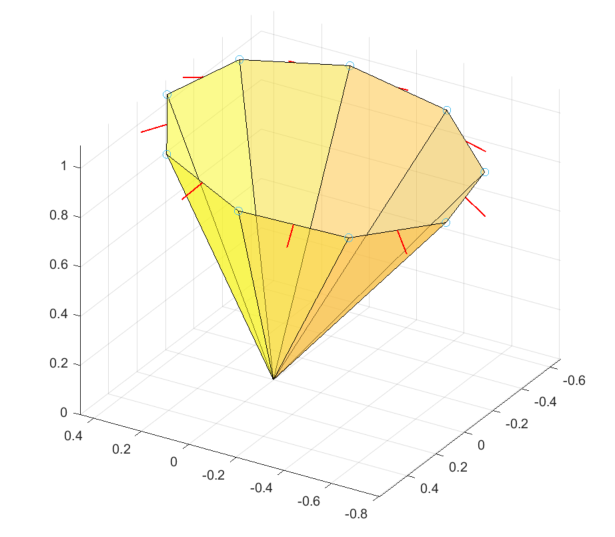
\includegraphics[width=0.7\linewidth]{approx}
%			\caption{}
			\label{fig:approx}
		\end{figure}
		
		
	\end{flushleft}
\end{frame}


\begin{frame}{Under- and over-approximation, 1}
	% \framesubtitle{Parameter estimation}
	\begin{flushleft}
		
		When approximating friction cone, we aim to retain some of the properties of the original geometry. 
		
		\bigskip
		
		\emph{Under-approximation} (inner approximation) implies that the approximate cone $\mathcal{C}_a$ lies inside the original cone $\mathcal{C}$. Meaning any point  $\bo{x} \in \mathcal{C}_a$ is also in $\mathcal{C}$, but $\exists \bo{y}: \bo{y} \in \mathcal{C}, \bo{y} \notin \mathcal{C}_a$.
		
		\bigskip
		
		\emph{Over-approximation} (outer approximation) implies that the original cone $\mathcal{C}$ lies inside the approximate cone $\mathcal{C}_a$. Meaning any point  $\bo{x} \in \mathcal{C}$ is also in $\mathcal{C}_a$, but $\exists \bo{y}: \bo{y} \in \mathcal{C}_a, \bo{y} \notin \mathcal{C}$.
		
		\bigskip
		
		Usually we assume that approximation is as tight as possible, given number of faces allocated for the approximate cone $\mathcal{C}_a$.
		
	\end{flushleft}
\end{frame}


\begin{frame}{Under- and over-approximation, 2}
	% \framesubtitle{Parameter estimation}
	\begin{flushleft}
		
		
		
		% TODO: \usepackage{graphicx} required
		\begin{figure}
			\centering
			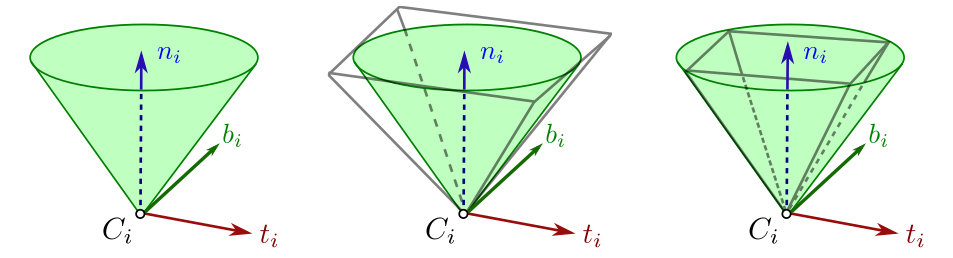
\includegraphics[width=0.9\linewidth]{InnerOuter}
			\caption{Original cone, inner and outer approximations. \bref{https://scaron.info/robotics/friction-cones.html}{Image credit.}}
			\label{fig:innerouter}
		\end{figure}
		
		
	\end{flushleft}
\end{frame}


\begin{frame}{H-representation, 1}
	% \framesubtitle{Parameter estimation}
	\begin{flushleft}
		
		One of the ways to encode a linearized friction cone is H-representation - presenting the polytope as a collection of linear inequalities, which represent faces of the polytope. Let us compare cone and H-polytope as sets:
		
		\bigskip
		
		\begin{itemize}
			\item $\mathcal{C} = \{ \bo{x}: \ || (\bo{I} - \bo{n}\bo{n}\T) \bo{f}_R ||
			\leq \mu \bo{n}\T \bo{f}_R \},$ - cone;
			
			\item $\mathcal{C}_a = \{ \bo{x}: \ \bo{A}\bo{x} \leq \bo{b} \},$ - H-polytope.
		\end{itemize}
		
		
	\end{flushleft}
\end{frame}

\begin{frame}{H-representation, 2}
	% \framesubtitle{Parameter estimation}
	\begin{flushleft}
		
		There are many way to generate matrix $\bo{A}$ and vector $\bo{b}$ in H-representation. 
		
		\bigskip
		
		Assuming the only restriction imposed on the normal reaction force is its positive value (it pushes and not pulls on the ground), all faces of the friction polytope pass through the origin. Each face lies on a boundary of  halfspace represented as:
		
		\begin{equation}
			\bo{a}_i\T \bo{x} \leq b_i
		\end{equation}
		%
		where $\bo{a}_i$ is the $i$-th row of the matrix $\bo{A}$. The Plane of which the face lies is represented by equality $\bo{a}_i\T \bo{x} \leq b_i$. But since $\bo{x} = 0$ lies on each of these faces, it implies $\bo{b} = \bo{0}$.
		
	\end{flushleft}
\end{frame}



\begin{frame}{H-representation, 3}
	% \framesubtitle{Parameter estimation}
	\begin{flushleft}
		
		The key requirement in generating friction polytope is doing it with less computation. One of the ways to do it is by starting with generating a number of equally spaced points $\bo{v}_i$ on a level set of the cone (such that $\bo{n}\T\bo{v}_i = \bo{n}\T\bo{v}_j \ \forall i,j$). 
		
		\bigskip
		
		We can describe a plane passing through points $\bo{0}, \bo{v}_i, \bo{v}_{i+1}$ by its normal vector $\bo{m}_i$:
		
		\begin{equation}
			\bo{m}_i = \bo{v}_i \times \bo{v}_{i+1}
		\end{equation}
		
		These normals $\bo{n}_i$ are equivalent to $\bo{a}_i$ up to a sign. To make sure the vectors are pointed "out" of the cone, we can use the following trick:
		
		\begin{equation}
			\bo{a}_i = \bo{m}_i \ \text{sign}(\bo{m}_i\T \bo{P}(\bo{v}_i + \bo{v}_{i+1}))
		\end{equation}
		
		
	\end{flushleft}
\end{frame}



\begin{frame}{H-representation, 4}
	% \framesubtitle{Parameter estimation}
	\begin{flushleft}
		
		Sometimes we want to add limits of minimum and maximum normal reaction force, e.g. to avoid forces that test the limits of our friction models. This can be done by appending the following inequalities to our H-representation:
		
		
		\begin{align}
			\bo{n}\T \bo{x} \leq f_{\text{max}}
			\\
			-\bo{n}\T \bo{x} \leq -f_{\text{min}}
		\end{align}
		
		
	\end{flushleft}
\end{frame}



\begin{frame}{V-representation}
	% \framesubtitle{Parameter estimation}
	\begin{flushleft}
		
		Alternatively we could use \emph{vertex representation} of a friction cone, that requires a friction force to lie inside a polytope generated as a convex combination of its vertices $\bo{v}_1, \ \bo{v}_2, \ ...$; Unlike in the previous example, these should include the origin.
		
		\bigskip
		
		We can represent such polytope as a set in the following way:
		
		\begin{align}
			\mathcal{C}_a = \{ \bo{x}: \ \bo{x} = \sum \alpha_i \bo{v}_i; \  \sum \alpha_i = 1; \ \alpha_i \geq 0\}
		\end{align}
		
		
		
	\end{flushleft}
\end{frame}



\begin{frame}{V-rep vs H-rep}
	% \framesubtitle{Parameter estimation}
	\begin{flushleft}
		
		\begin{itemize}
			\item In H-rep solving containment problem comes to evaluating linear inequalities. In V-rep solving containment problem requires solving an optimization problem.
			
			\item V-rep naturally handles upper limit on normal reaction force; in fact, the choice of vertices "height" determines the upper limit.
			
			\item V-rep skips the step of constructing the half-space normal.
		\end{itemize}
		
	\end{flushleft}
\end{frame}



\begin{frame}{V-representation without a cap, 1}
	% \framesubtitle{Parameter estimation}
	\begin{flushleft}
		
		We can lift the cap on the maximum normal reaction by excluding the condition $\sum \alpha_i = 1$:
		%
		\begin{align}
			\mathcal{C}_a = \{ \bo{x}: \ \bo{x} = \sum \alpha_i \bo{v}_i; \ \alpha_i \geq 0\}
		\end{align}
		%
		Assume that $\bo{v}_1 = 0$ and $\bo{v}_i, \forall i \neq 1$ lie on a level-set, meaning $\bo{n}\T\bo{v}_i = h, \ \forall i \neq 1$. Let us consider the subset $\mathcal{C}_d$:
		%
		\begin{align}
			\mathcal{C}_d = \{ \bo{x}: \ \bo{x} = \sum \alpha_i \bo{w}_i; \  \sum \alpha_i = 1;  \ \alpha_i \geq 0\}
		\end{align}
		%
		where $\bo{w}_i = k \bo{v}_i$. Defining $\beta_i = k \alpha_i$:
		%
		\begin{align}
			\mathcal{C}_d = \{ \bo{x}: \ \bo{x} = \sum \beta_i \bo{v}_i; \  \sum \beta_i = k;  \ \beta_i \geq 0\}
		\end{align}
	
		We can see that choice of $k$ decided the size of $\mathcal{C}_d$; without the constraint $\sum \alpha_i = 1$ (and hence $\sum \beta_i = k$) we get a set $\mathcal{C}_a$ which is a union of all sets $\mathcal{C}_d$.
		
	\end{flushleft}
\end{frame}




\begin{frame}{Example}
	% \framesubtitle{Parameter estimation}
	\begin{flushleft}
		
		A simple example of linear approximation of a friction cone is:
		
		\begin{equation}
			\begin{cases}
				|f_{\tau, 1}| \leq \mu f_n \\
				|f_{\tau, 2}| \leq \mu f_n
			\end{cases}
		\end{equation}
		
		This approximation has 4 faces.
		
	\end{flushleft}
\end{frame}



\begin{frame}{Read more}
	\begin{itemize}
		\item Friction cones, notes by St\'ephane Caron. \bref{https://scaron.info/robotics/friction-cones.html}{scaron.info/robotics/friction-cones.html}
		 
	\end{itemize}
\end{frame}



\myqrframe

\end{document}
